% ドキュメントの設定
\documentclass[a4paper,11pt,xelatex,ja=standard]{bxjsarticle}
\usepackage{tikz}
\usetikzlibrary {datavisualization.formats.functions}
\usepackage{pgfplots}
\usepackage{float}
\usepackage{amsmath}

% ドキュメント開始
\begin{document}

\section{実験の目的}

    \begin{enumerate}
        \item 2種類の単電源オペアンプを用いて回路を製作し、入出力Rail to Railとそうではないものの違いについて実験を通して確認する。
        \item コンパレータ回路を製作しコンパレータとしての動作、コンパレータを用いたPWM信号生成における動作・原理について検証する。
    \end{enumerate}

\section{実験の作業順序}

    \begin{enumerate}
        \item コンパレータ回路の製作:
            \begin{itemize}
                \item 単電源オペアンプ(NJU7043,NJM2904)を使用して、図1のようなコンパレータ回路を作成する。
                \item 非反転入力端子(V+)に入力信号を、反転入力端子(V-)に炭素抵抗2本で分圧された基準電圧(Vref)を入力する。Vrefは表1に基づいて設計し、E24系列の抵抗を使用する。実際のVrefを記録する。
            \end{itemize}
        \item コンパレータの評価:
            \begin{itemize}
                \item 製作した回路にVP-P=VDD(誤差+0.0V,-0.3V)、周波数=【出席番号】kHzの正弦波を入力し、正弦波と基準電圧、正弦波とコンパレータ出力をオシロスコープで観測して動作を評価する。ファンクションジェネレータは0V以上、VDD以下の電圧を印加するように調整する。
            \end{itemize}
        \item 三角波による評価:
            \begin{itemize}
                \item 反転入力端子に正弦波の振幅100~90、周波数1/10に設定した三角波を入力し、同様に計測してコンパレータの動作を評価する。出力波形の特徴について考察する。
            \end{itemize}
        \item 可変抵抗による評価:
            \begin{itemize}
                \item 非反転入力端子に10kΩの半固定抵抗器を接続し、非反転入力端子、反転入力端子間の入力関係、三角波とコンパレータ出力を観測し動作を評価する。
            \end{itemize}
        \item 温度センサによる評価:
            \begin{itemize}
                \item 反転入力端子にMCP9701を接続し、室温(T0)および触れたとき(T1)の入力電圧をデジタルテスタで計測する。
            \end{itemize}
        \item 温度変化によるDCファンの動作:
            \begin{itemize}
                \item 温度変化により動作点が来るように分圧抵抗を設計し、DCファンが動作する回路を完成させて動作を検証する。DCファンはトランジスタ2SC1815を用いて駆動する。
            \end{itemize}
    \end{enumerate}

\section{実験の結果}
    \subsection{コンパレータの評価}

        製作した回路にVP-P=VDD(誤差+0.0V,-0.3V)、周波数=【出席番号】kHzの正弦波を入力し、正弦波と基準電圧、正弦波とコンパレータ出力をオシロスコープで観測した結果を以下に示す。その結果、正弦波の瞬時値が基準電圧を超えた瞬間にコンパレータの出力が0Vから5Vに上昇した。このことからコンパレータが正しい動作をしていることがわかった。

        \begin{figure}[H]
            \centering
            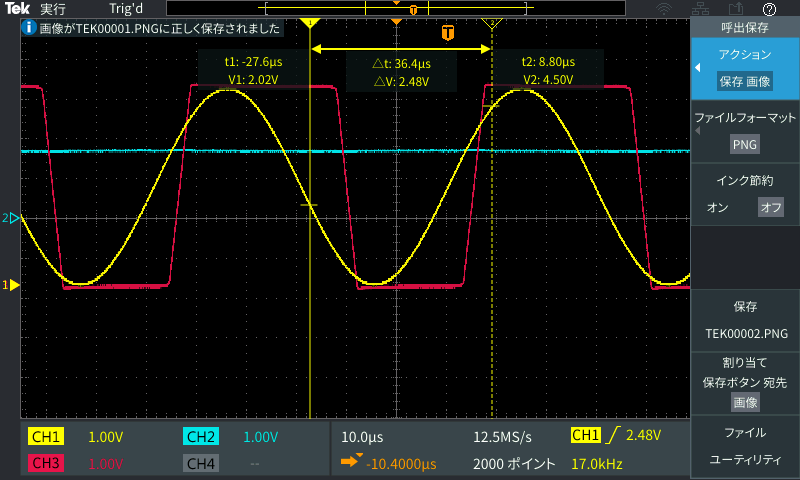
\includegraphics[width=0.5\textwidth]{./img/24-6-1/3.png}
            \caption{正弦波と基準電圧、正弦波とコンパレータ出力}
        \end{figure}

    \subsection{三角波による評価}
        反転入力端子に正弦波の振幅100~90、周波数1/10に設定した三角波を入力し、同様に計測した結果を以下に示す。三角波と正弦波を入力するとDuty比が異なる波がコンパレターから出力されていることを確認できた。

        \begin{figure}[H]
            \centering
            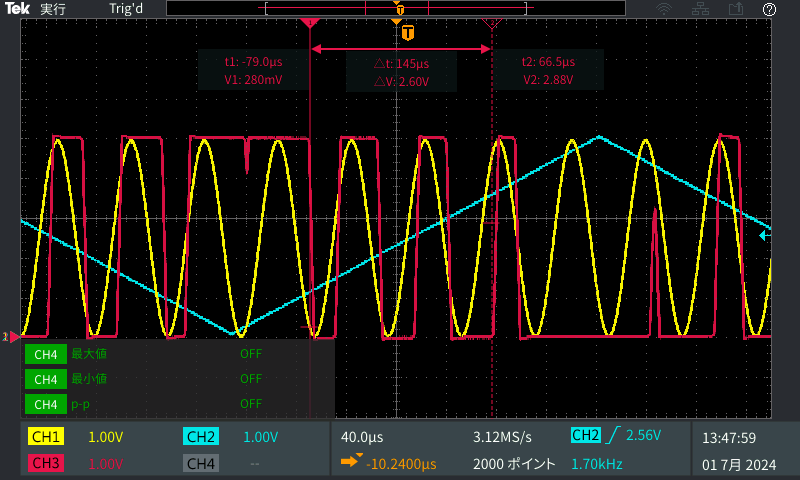
\includegraphics[width=0.5\textwidth]{./img/24-6-1/4.png}
            \caption{反転入力端子に正弦波の振幅100~90、周波数1/10に設定した三角波を入力し、同様に計測した結果}
        \end{figure}

\section{実験の考察およびまとめ}

        \subsection{コンパレータ回路の評価}
        今回の実験では、コンパレータ回路の基本動作を確認するために、正弦波および三角波を入力信号として使用しました。実験結果から、以下のことがわかりました。
        
        \begin{itemize}
            \item 正弦波の入力に対して、コンパレータは基準電圧を超えた瞬間に出力を変化させ、適切なスレッショルド検出機能を示しました。このことは、コンパレータが信号のゼロクロッシングポイントを正確に検出できることを意味します。
            \item 三角波の入力に対しては、出力波形のDuty比が入力信号に依存して変化することが確認されました。これにより、コンパレータがPWM信号生成の基本動作を適切に行っていることが示されました。
        \end{itemize}
        
        これらの結果は、コンパレータ回路が期待通りの動作をすることを示しており、回路設計の妥当性を確認することができました。
        
        \subsection{温度センサによる評価}
        MCP9701温度センサを使用した評価では、温度変化に対するセンサの出力電圧の変動を確認しました。
        
        \begin{itemize}
            \item 室温(T0)と触れたとき(T1)の入力電圧を測定した結果、センサの出力が温度に応じて適切に変化することが確認されました。これにより、温度センサが正しく機能していることが示されました。
            \item この特性を利用して、温度変化に応じたDCファンの動作を実現する回路を設計し、温度変化によるファンのオン/オフ制御が適切に行われることを確認しました。
        \end{itemize}
        
        \subsection{まとめ}
        本実験を通して、コンパレータ回路および温度センサを用いた応用回路の基本的な動作を確認することができました。特に、コンパレータのスレッショルド検出機能やPWM信号生成の能力、および温度センサを用いた温度制御の可能性について理解を深めることができました。
        
\end{document}
